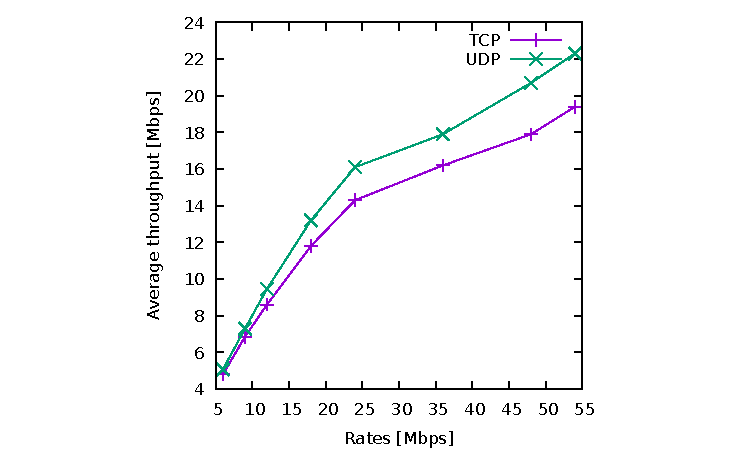
\includegraphics[width=0.5\textwidth]{traces/L3-1-4-tput.pdf}
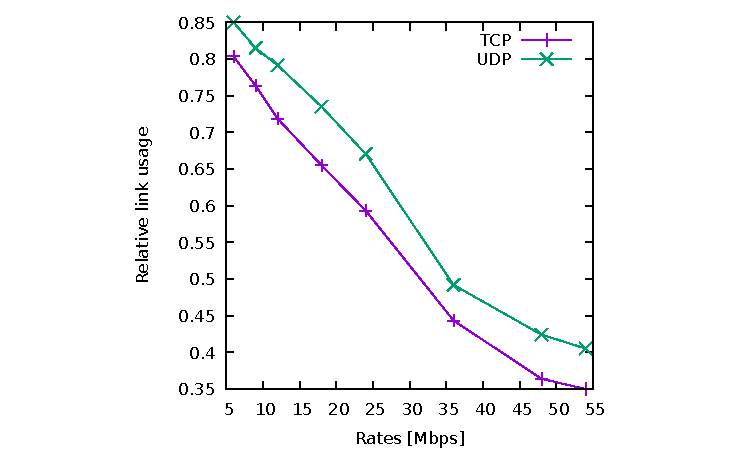
\includegraphics[width=0.5\textwidth]{traces/L3-1-4-usage.pdf}
UDP's throughput is consistenly higher than TCP's. TCP has larger headers so more overhead. More importantly, TCP's congestion control mechanisms lead to reduced throughput. Throughput grows together with bitrate: the network supports sending more bits per second with higher bitrates. \\ \\
The throughput does not grow as quickly as the bitrate: with higher bitrates the bits are sent faster and bits are more likely to get lost. Due to this additional loss doubling the bitrate does not double the observed throughput. This translates to a decreasing usage with increasing bitrate.
